\begin{figure}[!p]
    \centering
    \begin{subfigure}[b]{\SideBySidePlotWidth}
        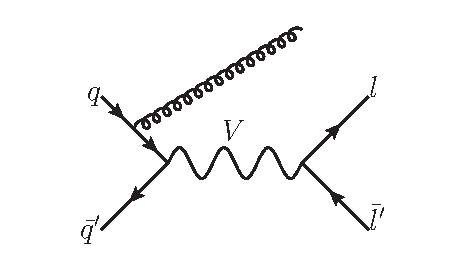
\includegraphics[width=\linewidth]{figures/TheoryFigures/VectorBosonQToLeptonGJet.eps}
        \caption{}
        \label{fig:feyn_DYISR}
    \end{subfigure}%
    \begin{subfigure}[b]{\SideBySidePlotWidth}
        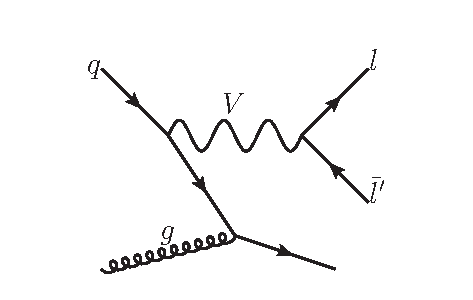
\includegraphics[width=\linewidth]{figures/TheoryFigures/VectorBosonQToLeptonqJet.eps}
        \caption{}
        \label{fig:feyn_DYQuarkRadiation}
    \end{subfigure}%
    \hfill
    \begin{subfigure}[b]{\SideBySidePlotWidth}
        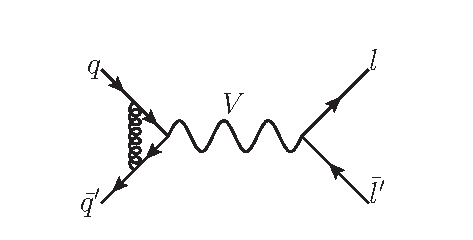
\includegraphics[width=\linewidth]{figures/TheoryFigures/VectorBosonQToLeptonqgexchange.eps}
        \caption{}
        \label{fig:feyn_DYloops}
    \end{subfigure}%
    \begin{subfigure}[b]{\SideBySidePlotWidth}
        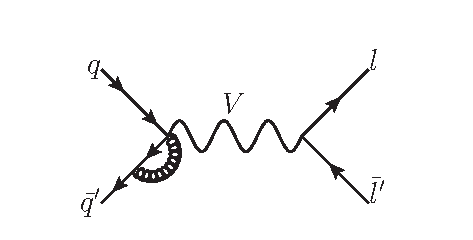
\includegraphics[width=\linewidth]{figures/TheoryFigures/VectorBosonQToLeptonqLoop.eps}
        \caption{}
        \label{fig:feyn_DYmoreloops}
    \end{subfigure}%

    \caption[
        Higher order DY Feynman diagrams.
    ]{
        Higher order DY Feynman diagrams. a is an example of when an incoming quark radiates a gluon. In b the quark radiates a \Z before interacting with a gluon. In both c and d the gluons interact with the quarks but are not radiated.
    }
    \label{fig:higher_order_z_diagrams}
\end{figure}